\documentclass{beamer}
\usefonttheme[onlymath]{serif}

\usepackage[utf8]{inputenc}
\usepackage[english]{babel}
\usepackage{amsmath}
\usepackage{xcolor}
\usepackage{amsthm}
\usepackage{amsfonts}
\usepackage{amssymb}
\usepackage{mathtools}
\usepackage{tikz}
\usepackage{graphicx}
\usetikzlibrary{arrows, automata, graphs, shapes, decorations.pathreplacing, decorations.pathmorphing}

% define environments
%\renewcommand{\labelenumi}{(\roman{enumi})}
\newcommand{\equalhat}{\mathrel{\widehat{=}}}
\DeclareMathOperator{\spn}{span}

\newtheorem{thm}{Theorem}
\newtheorem{lem}{Lemma}

\definecolor{proof}{HTML}{75008C}
\definecolor{def}{HTML}{0000FF}
\definecolor{remark}{HTML}{389A39}
\definecolor{highlight}{HTML}{CE9E00}
\definecolor{grey}{HTML}{666666}
\newcommand{\defi}[1]{{\color{def}#1}}

% theme
\usetheme{Boadilla}
\useinnertheme{circles}
\setbeamertemplate{blocks}[rounded][shadow=false]
\setbeamercolor{block title}{fg=white, bg=blue!70}
\setbeamercolor{block body}{fg=black, bg=blue!15}
\beamertemplatenavigationsymbolsempty

% title page
\title[Übung 4]{FoSAP - Übung 4}
%\subtitle[Seminar on Mathematical Optimization]{Seminar on Mathematical Optimization in Summer Term 2017}
%\author[Niklas Rieken]{Niklas Rieken}
%\institute[RWTH Aachen]{RWTH Aachen}
%\date{June 13, 2017}
%\logo{\pgfimage[width=2cm,height=2cm]{}}
%\titlegraphic{\includegraphics[width=2cm,height=2cm]{}}
%\subject{}
%\keywords{}

% and here we go
\begin{document}

\begin{frame}{Aufgabe T13}
	Minimiere den DFA und finde einen regulären Ausdruck, der seine Sprache beschreibt:
	\begin{figure}
		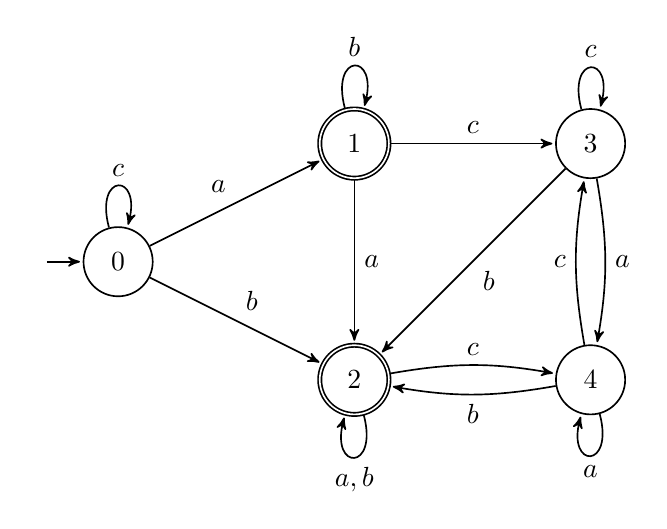
\begin{tikzpicture}[->, >=stealth', shorten >=1pt, auto, node distance=2.8cm, semithick]
			\node[initial, initial text=, state]	(0)	at (0, 0)	{$0$};
			\node[state, accepting]				(1) at (3, 1.5)	{$1$};
			\node[state, accepting]				(2) at (3, -1.5)	{$2$};
			\node[state]							(3) at (6, 1.5)	{$3$};
			\node[state]							(4) at (6, -1.5)	{$4$};

			\path	(0) edge node {$a$} (1)
					(0) edge node {$b$} (2)
					(0) edge[loop above] node {$c$} (0)
					(1) edge node {$a$} (2)
					(1) edge[loop above] node {$b$} (1)
					(1) edge node {$c$} (3)
					(2) edge[loop below] node {$a, b$} (2)
					(2) edge[bend left=10] node[above] {$c$} (4)
					(3) edge[bend left=10] node[right] {$a$} (4)
					(3) edge node {$b$} (2)
					(3) edge[loop above] node {$c$} (1)
					(4) edge[loop below] node {$a$} (4)
					(4) edge[bend left=10] node[below] {$b$} (2)
					(4) edge[bend left=10] node[left] {$c$} (3);
		\end{tikzpicture}
	\end{figure}
\end{frame}

\begin{frame}{Die Goldbach'sche Vermutung} 
	\begin{itemize}
		\item Wir wissen: \( L, K \) regulär \( \implies L \cdot K \) regulär.\pause
		\item Gilt die Umkehrung? \( L \cdot K \) regulär \( \implies  L \) und \( K \) regulär?\pause
		\item Kontraposition: \( L, K \) nicht regulär \( \implies L \cdot K \) nicht regulär.\pause
		\item Dann mit \( L = \{ a^p \mid p > 2 \text{ prim} \} \) (nicht regulär!!):\pause\\
		Goldbach'sche Vermutung:
		\[
			L^2 = L \cdot L \overset{\text{?}}{=} \{ a^{2n} \mid n > 2 \} 
		\]
	\end{itemize}
\end{frame}

% eof
\end{document}